\chapter{Automatisation de la maison}

\section{L’intelligence des objets}
	\subsection{Définition d’un objet connecté}
Aujourd'hui les objets connectés font partis de notre quotidien, et peuvent réaliser énormément 
d'actions différentes. Globalement on peut dire qu'un objet connecté, ou l'internet des objets, représente 
l'extension d'Internet à l'ensemble des objets de notre monde physique. Cela permet de donner de 
l'intelligence à des objets, afin qu'ils puissent nous communiquer différentes informations 
(\textbf{Capteurs}), ou bien exécuter différentes choses (\textbf{Actionneurs}). Ces événements peuvent être 
réalisés manuellement ou automatiquement selon le besoin.

Malgré tout, ces objets ne sont sémantiquement pas connectés entre eux pour plein de raisons différentes. 
SmartDevCom permet de réaliser un ensemble d'objet tous connectés entre eux. Un objet connecté est constitué 
d'un ou plusieurs capteur(s) ou actionneur(s).
% 		Définition générale + notre version par rapport au projet
	\subsection{Les capteurs}
	
Les capteurs sont tous les objets qui permettent d'obtenir une information sur l'environnement. Ces capteurs 
permettent par exemple de connaître la température de la pièce, de savoir si la lumière est allumée, ou si la 
porte d'entrée est ouverte.

Ces capteurs permettent une interaction simpliste avec l'environnement puisqu'ils permettent seulement 
d'obtenir une information physique. Ainsi, l'utilisation d'un capteur est très simple, puisqu'il suffit de 
lui demander d'envoyer la valeur qu'il contient.
% 		les types de capteurs
% 		leurs caractéristiques au sein d’un objet connecté
	\subsection{Les actionneurs}
	
Les actionneurs sont tous les objets qui permettent de réaliser une action. Ces actionneurs permettent par 
exemple d'ouvrir les volets, d'allumer la climatisation, ou bien d'allumer la lumière.

Ils permettent une interaction plus prononcée avec l'environnement, comparativement aux capteurs, étant donné 
qu'ils ont besoin de paramètres pour réaliser l'action voulue. Par exemple si l'on souhaite allumer une 
lumière intelligente, il faudra préciser l'intensité lumineuse, ainsi que la couleur de celle-ci.
% 		les types de capteurs
% 		leurs caractéristiques au sein d’un objet connecté

\section{La communication des objets}
	\subsection{Présentation des technologies de communication}
Actuellement, il existe de nombreux protocoles réseaux qui permettent la communication entre les différents 
objets. Ces protocoles établissent des normes, afin de pouvoir dialoguer entre différents acteurs.

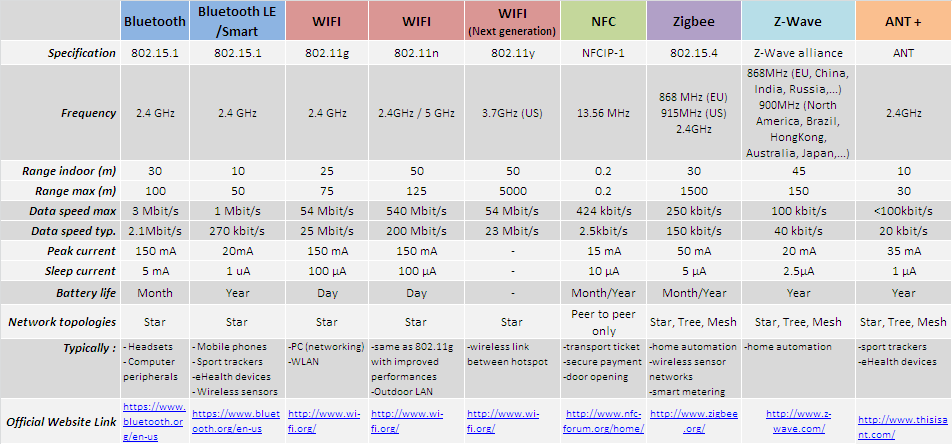
\includegraphics{img/tableau-total.png} 

Tous ces protocoles ont leur avantages et leur inconvénients. Malgré tous ces protocoles, on peut voir qu'il 
existe principalement deux familles :

\paragraph{Les protocoles très énergivores}qui permettent de faire transiter des données avec un débit très 
élevé. Cette cadence est permise grâce à une fréquence trés élevé. Cette fréquence a par conséquent 
l'inconvénient de très peu passer les obstacles, et donc d'émettre sur une courte distance.

\paragraph{Les protocoles peu énergivores}qui possèdent des caractéristiques opposées. En effet ils 
permettent de faire transiter des données avec un faible débit, sur une grande distance grâce à une fréquence 
bien moindre.

C'est donc la deuxième famille qui est la plus utilisée pour l'internet des objets, puisqu'ils n'ont pas 
besoin d'envoyer beaucoup de données, ont besoin d'envoyer le plus loin possible, et surtout d'avoir le plus 
d'autonomie possible. Les protocoles les plus réprésentatifs de cette famille, sont le Bluetooth Low Energy 
(ou BLE), le Zigbee, et Z-Wave. Ces deux derniers sont relativement onéreux et compliqués à mettre en place, 
c'est pourquoi le BLE est le protocole le plus démocratisé de cette famille.

% 		wifi, bluetooth, BLE, zig-bee, …
% 		quelques caractéristiques (débit, portée, consommation)
	\subsection{Les différentes topologies de réseaux}
En plus des différents protocoles, il existe aussi des topologies différentes pour créer un réseau d'objets. 
La topologie d'un système représente la manière dont celui-ci est organisé est agencé. Ainsi en fonction des 
besoins, tout comme pour les protocoles, une topologie sera plus adéquat qu'une autre.

	    \subsubsection{Etoile}
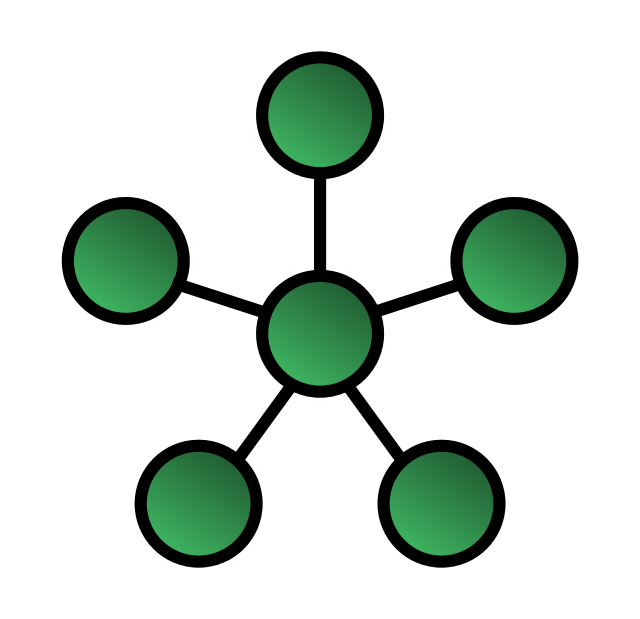
\includegraphics{img/StarNetwork.svg.png}
C'est la topologie la plus commune dans les communications. Elle est aussi appelée l'architecture 
client/serveur dans le sens où il y une machine qui dirige tout le système, et par lequel toutes les données 
passent. Il s'agit de l'architecture la plus simple, puisqu'avec cette topologie, il est facile de changer de 
sortir du réseau local, et permet d'envoyer rapidement un paquet d'un noeud à un autre.

	    \subsubsection{P2P}
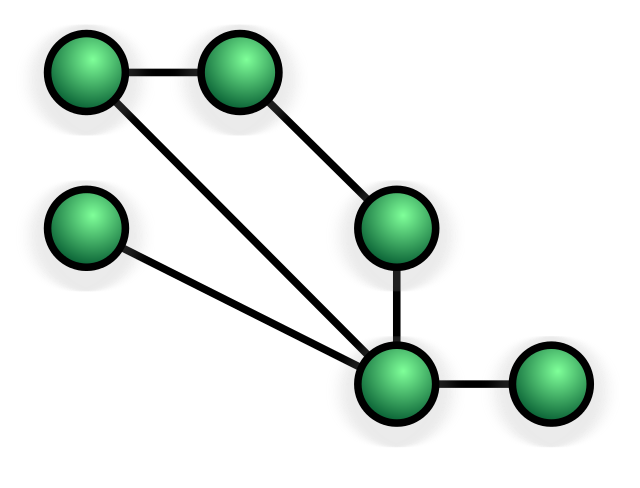
\includegraphics{img/NetworkTopology-Mesh.svg.png}
Cette topologie, aussi appelé réseau meshé, permet d'avoir une architecture réseau plus robuste, puisqu'il 
existe plusieurs chemins pour arriver à un noeud. Elle donne aussi une plus grande securité au niveau de 
l'acheminement des paquets, puisque toutes les données ne passent pas au même endroit, il est donc plus 
difficile de les sniffer. Pour finir cette architecture permet d'avoir un réseau beaucoup plus grand et 
dynamique, puisqu'il n'existe pas de noeud central. L'inconvénient de cette architecture est qu'elle est plus 
dure à mettre en place, du fait qu'il existe plusieurs routes pour acheminer les données. De ce fait, il faut 
gérer la duplication possible des paquets, et le routage dynamique si un des noeud n'est plus fonctionnel.

	    \subsubsection{Arbre}
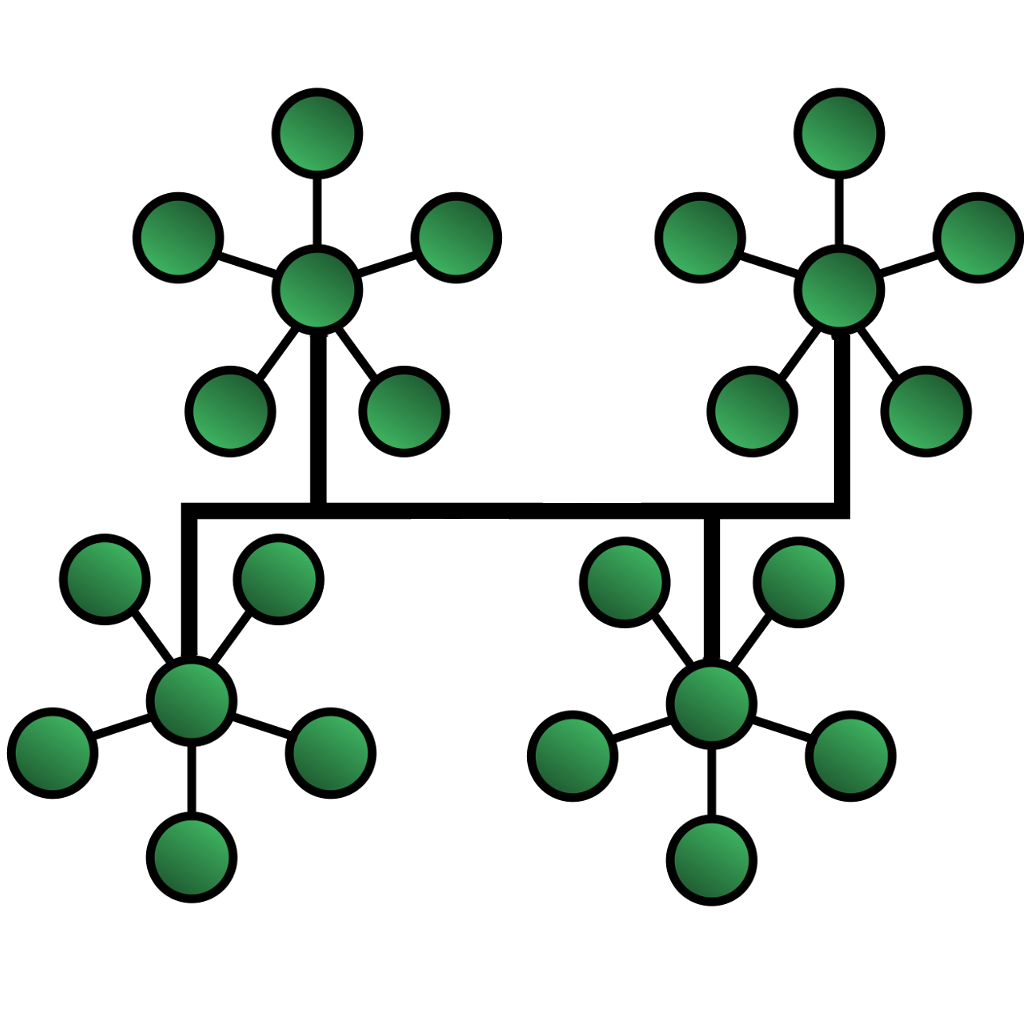
\includegraphics{img/TreeTopology.png}
Cette architecture est simplement l'extension du réseau étoile, c'est l'architecture utilisée par Internet.
% 		p2p, étoile, mesh, ...
% 		lien avec les technos
	\subsection{Application du réseau à la domotique}


% 		les technologies les plus adaptées à la domotique
% 		exemples d’architecture réseau dans une maison (avec ou sans mélange de technos)

\section{La centralisation de l’intelligence : Jarvis}
	\subsection{Vision macroscopique d’un système domotique}
Actuellement, la croissance de l'intégration des objets connectés dans notre quotidien est réellement forte. 
Dans un futur proche, nous seront entourés par un très grand nombre de ces objets. Mais il n'existe peu de 
systèmes aujourd'hui qui permettent une interaction intelligente avec l'ensemble de ces objets. Il existe peu 
de moyens simples et directs de réussir à communiquer avec l'ensemble de ces objets connectés sans devoir se 
connecter manuellement à eux. De plus tous ces acteurs utilisent un langage différent pour communiquer, il 
est donc difficile de réussir à centraliser un moyen de communication universel.

SmartDevCom permet de réaliser une intelligence semblable à Jarvis, qui est une intelligence artificielle 
forte, que l'on peut voir dans les films Iron Man. Cette intelligence peut communiquer avec tout, et peut 
même deviner ce qu'elle doit faire à partir d'informations qu'elle aura apprise elle-même au cours du temps. 
Avec le temps, Jarvis est capable d'apprendre est de réaliser des tâches complexes : Les scenarios.
% 		les conséquences de la connexion des objets
	\subsection{Les scénarios}
Les scénarios sont un ensemble d'actions que l'on souhaite faire en simultannée et/ou de manière 
séquentielle. 
Par exemple, lorsque l'on souhaite regarder un film, voici un scénario avancé que l'on pourrait réaliser :
\begin{itemize}
 \item Choix du film
 \item Choix du volume
 \item Fermeture des stores
 \item Extinction de la lumière principale
 \item Allumage petite lumière tamisée, accordée au thème du film
 \item Passage du téléphone en mode silencieux 
\end{itemize}

Grâce au système de scénario, il serait possible de réaliser l'intégralité des tâches, seulement en demandant 
de lancer le film voulu. Nous allons voir comment créer ce genre de scénario
% 		explication sur l’intérêt de la connexion des objets
% 		exemples d’utilisations
	\subsection{Analyse et anticipation de requêtes}
Afin de créer l'intelligence des objets, l'utilisateur possède deux choix. Il peut créer un scénario 
manuellement en indiquant les tâches à réaliser parrallèlement et séquentiellement. Ou alors il peut laisser 
l'apprentissage se faire. En effet, Jarvis peut simplement faire une étude statistique des utilisations des 
objets, et faire une corrélation entre eux. Ainsi il peut voir après plusieurs utilisations, que 
lorsque l'utilisateur réalise une tâche, il en réalise forcément d'autres. Ceci permet donc de réaliser 
une intelligence centrale, capable d'être personnalisé automatiquement pour son utilisateur, et de pouvoir 
réaliser un ensemble de tâche de manière autonome.
% 		analyse plus poussée des données : statistiques, interprétations des mesures
% 		intégration d’intelligence artificielle
% 		exécution de tâches de façon autonomes
% 		les limites
